\documentclass{article}
\usepackage{tikz}
\usepackage{amsmath}
\usetikzlibrary{calc,patterns,angles,quotes,positioning}
\begin{document}

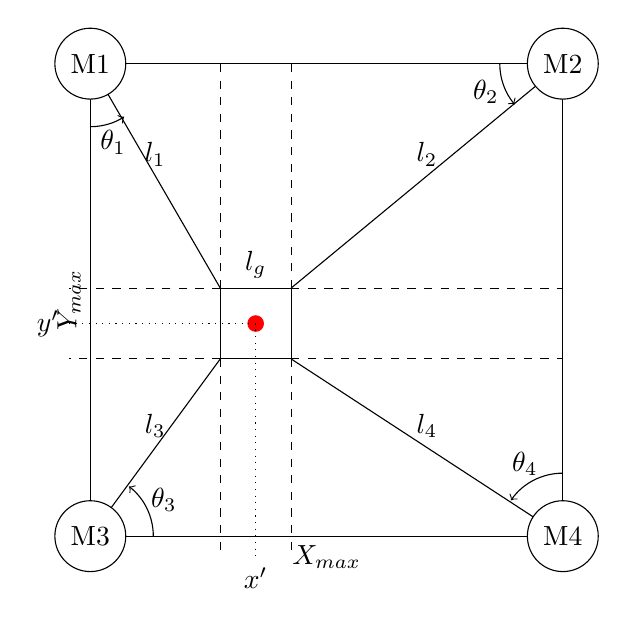
\begin{tikzpicture}[scale=1.5]

\def\gripSize{0.3}
%\pgfmathsetmacro{\grip_size}{0.3}

\coordinate (M1) at (0,4);
\coordinate (M2) at (4,4);
\coordinate (M3) at (0,0);
\coordinate (M4) at (4,0);

\draw (M3)--(M4) node[midway,below] (xaxis) {$X_{max}$};
\draw (M4)--(M2) node[midway,above](yaxisr){};
\draw (M1)--(M2) node[midway,right](xaxist){};
\draw (M3)--(M1) node[midway,above,sloped] (yaxis) {$Y_{max}$}  ;

%\draw (M3,M1) node (yaxis){};

\coordinate (c) at (1.4, 1.8);
\coordinate (c1) at ($(c) + (-\gripSize,\gripSize)$);
\coordinate (c2) at ($(c) + (\gripSize,\gripSize)$);
\coordinate (c3) at ($(c) + (-\gripSize,-\gripSize)$);
\coordinate (c4) at ($(c) + (\gripSize,-\gripSize)$);
\draw (c1) -- (0,4) node[midway,above] {$l_1$} ;
\draw (c2) -- (4,4) node[midway,above] {$l_2$} ;
\draw (c3) -- (0,0) node[midway,above] {$l_3$} ;
\draw (c4) -- (4,0) node[midway,above] {$l_4$} ;

%\draw ()
\fill[red] (c) circle (2pt);

\draw[dotted] (yaxis |- c) node[left] {$y'$}
    -| (xaxis -| c) node[below] {$x'$};
    
\draw[dashed] (c3) -- (xaxis -| c3) ;
\draw[dashed] (c3) -- (yaxis |- c3) ;

\draw[dashed] (c1) -- (xaxist -| c1) ;
\draw[dashed] (c1) -- (yaxis |- c1) ;

\draw[dashed] (c2) -- (xaxist -| c2) ;
\draw[dashed] (c2) -- (yaxisr |- c2) ;
\draw[dashed] (c4) -- (xaxis -| c4) ;
\draw[dashed] (c4) -- (yaxisr |- c4) ;

\draw (c1) -- (c2) node[midway,above] {$l_g$} -- (c4) -- (c3) -- cycle;

\draw[fill=white] (M1) circle (0.3cm) node[text=black] {M1};

\draw[fill=white] (M2) circle (0.3cm) node[text=black] {M2};

\draw[fill=white] (M3) circle (0.3cm) node[text=black] {M3};

\draw[fill=white] (M4) circle (0.3cm) node[text=black] {M4};



\pic [draw, angle radius=0.8cm, ->, "$\theta_1$", angle eccentricity=1.3] {angle = M3--M1--c};

\pic [draw, angle radius=0.8cm, ->, "$\theta_2$", angle eccentricity=1.3] {angle = M1--M2--c};

\pic [draw, angle radius=0.8cm, ->, "$\theta_4$", angle eccentricity=1.3] {angle = M2--M4--c};

\pic [draw, angle radius=0.8cm, ->, "$\theta_3$", angle eccentricity=1.3] {angle = M4--M3--c};

\end{tikzpicture}
\linebreak

Inverse Kinematics:

\begin{equation}
\begin{aligned}
&X = \frac{X_{max}}{2} + \frac{l_3{}^2 - l_4{}^2}{2\left(X_{max} - l_g\right)}\\
&Y = \frac{Y_{max}}{2} + \frac{l_3{}^2 - l_4{}^2}{2\left(Y_{max} - l_g\right)}\\
\end{aligned}
\end{equation}

Forward Kinematics:

\begin{equation}
\begin{aligned}
&l_1 = \sqrt{\left(X - \frac{l_g}{2}\right)^2 + \left(Y_{max}-Y+\frac{l_g}{2}\right)^2}\\
&l_2 = \sqrt{\left(X_{max}-X+\frac{l_g}{2}\right)^2 + \left(Y_{max}-Y+\frac{l_g}{2}\right)^2}\\
&l_3 = \sqrt{\left(X-\frac{l_g}{2}\right)^2 + \left(Y-\frac{l_g}{2}\right)^2}\\
&l_4 = \sqrt{\left(X_{max}-X+\frac{l_g}{2}\right)^2 + \left(Y-\frac{l_g}{2}\right)^2}\\
\end{aligned}
\end{equation}

\end{document}